\section{Introduction}

\section{Change-based Models}

\section{Events}

\section{Model History}

\section{Optimisation Principles}


\subsection{The Last Value is All that Matters}
Lst. \ref{lst:set_attribute_eol} shows an EOL code to create a model. It performs set and unset operations to an attribute \texttt{name} of an object \texttt{node}. When executed, this code produces a CBP XML representation consists of 6 events shown in Lst. \ref{lst:set_attribute_cbp}. The 1\ts{st} event registers the package \texttt{node} and is followed by other events that create an object, with id "0", as an instance of a \texttt{Node} class (line 1) and then add the object to the model's resource to make the object a part of the model (line 2). The code then sets the attribute \texttt{name}'s value to "Old Name!" (line 3), then nullify/unset it (line 4), and finally sets it to "New Name!" as its latest value (line 5). Lst. \ref{lst:set_attribute_eol} shows that the last value's of \texttt{node.name} is all that matters (line 4). Any previous value assignment to the \texttt{name} attribute can be ignored (line 1 and 2), since the final version of the model will always be the same. 

\begin{lstlisting}[style=eol,caption={The EOL code for Setting  Attribute.},label=lst:set_attribute_eol]
var node = new Node;
node.name = "Old Name!";
node.name = null;
node.name = "New Name!";
\end{lstlisting}

\begin{lstlisting}[style=cbp-xml,caption={The generated change-based representation of Lst. \ref{lst:set_attribute_eol}. },label=lst:set_attribute_cbp]
0 <register epackage="node"/>
1 <create eclass="Node" epackage="node" id="0"/>
2 <add-to-resource position="0"><value eobject="0"/></add-to-resource>
3 <set-eattribute name="name" target="0"><value literal="Old Name!"/></set-eattribute>
4 <unset-eattribute name="name" target="0"/>
5 <set-eattribute name="name" target="0"><value literal="New Name!"/></set-eattribute>
\end{lstlisting}

All events that involve the object "0" are recorded in an object history. The object history records the line number of occurrence of each event (Lst. \ref{lst:set_attribute_eobject_history}). For example, \texttt{SetEAttributeValue} event contains line 3 and 5 based on its occurrence. 

\begin{lstlisting}[style=cbp-xml,caption={The event-line relationships recorded by an EObjectHistory of Lst. \ref{lst:set_attribute_eol}. },label=lst:set_attribute_eobject_history]
EObject: 0
    CreateEObjectEvent = [[1]]
    AddToResourceEvent = [[2]]
    EAttribute:
        name:
            UnsetEAttributeEvent = [[4]]
            SetEAttributeEvent = [[3], [5]]
\end{lstlisting}

The history enables us to track which lines can be ignored for optimisation so that not every event is executed to produce the same model. From Lst. \ref{lst:set_attribute_eobject_history}, we can deduce that line 3 and 4 can be ignored since the \texttt{SetEAttributeValue}'s last event always sets the end value of the \texttt{name} attribute. 

\begin{lstlisting}[style=cbp-xml,caption={The optimised change-based Representation of Lst. \ref{lst:set_attribute_eol}. },label=lst:set_attribute_optimised_cbp]
0 <register epackage="node"/>
1 <create eclass="Node" epackage="node" id="0"/>
2 <add-to-resource position="0"><value eobject="0"/></add-to-resource>
5 <set-eattribute name="name" target="0"><value literal="New Name!"/></set-eattribute>
\end{lstlisting}

\subsection{Unset Ignores Itself and Its Previous Sets and Unsets}

\begin{lstlisting}[style=eol,caption={The EOL code for Nullyfying/Unsetting  Attribute.},label=lst:unset_attribute_eol]
var node = new Node;
node.name = "Old Name!";
node.name = null;
node.name = "New Name!";
node.name = null;
\end{lstlisting}

\begin{lstlisting}[style=cbp-xml,caption={The generated change-based representation of Lst. \ref{lst:unset_attribute_eol}. },label=lst:unset_attribute_cbp]
0 <register epackage="node"/>
1 <create eclass="Node" epackage="node" id="0"/>
2 <add-to-resource position="0"><value eobject="0"/></add-to-resource>
3 <set-eattribute name="name" target="0"><value literal="Old Name!"/></set-eattribute>
4 <unset-eattribute name="name" target="0"/>
5 <set-eattribute name="name" target="0"><value literal="New Name!"/></set-eattribute>
6 <unset-eattribute name="name" target="0"/>
\end{lstlisting}

\begin{lstlisting}[style=cbp-xml,caption={The event-line relationships recorded by an EObjectHistory of Lst. \ref{lst:unset_attribute_eol}. },label=lst:unset_attribute_eobject_history]
EObject: 0
    CreateEObjectEvent = [[1]]
    AddToResourceEvent = [[2]]
    EAttribute:
        name:
            UnsetEAttributeEvent = [[4], [6]]
            SetEAttributeEvent = [[3], [5]]
\end{lstlisting}

\begin{lstlisting}[style=cbp-xml,caption={The optimised change-based Representation of Lst. \ref{lst:unset_attribute_eol}. },label=lst:unset_attribute_optimised_cbp]
0 <register epackage="node"/>
1 <create eclass="Node" epackage="node" id="0"/>
2 <add-to-resource position="0"><value eobject="0"/></add-to-resource>
\end{lstlisting}

\section{Performance}

\begin{lstlisting}[style=eol,caption={The EOL code for creating deep tree of nodes.},label=lst:deep_tree_eol]
var eRoot = new Node;
eRoot.name = "0";
for(i in Sequence{1..40}){
    var node = new Node;
    node.name = i.asString();
    eRoot.valNodes.add(node);
	   eRoot = node;
}
\end{lstlisting}

\subsection{Loading Deep Tree}
\begin{figure}[b!]
\centering
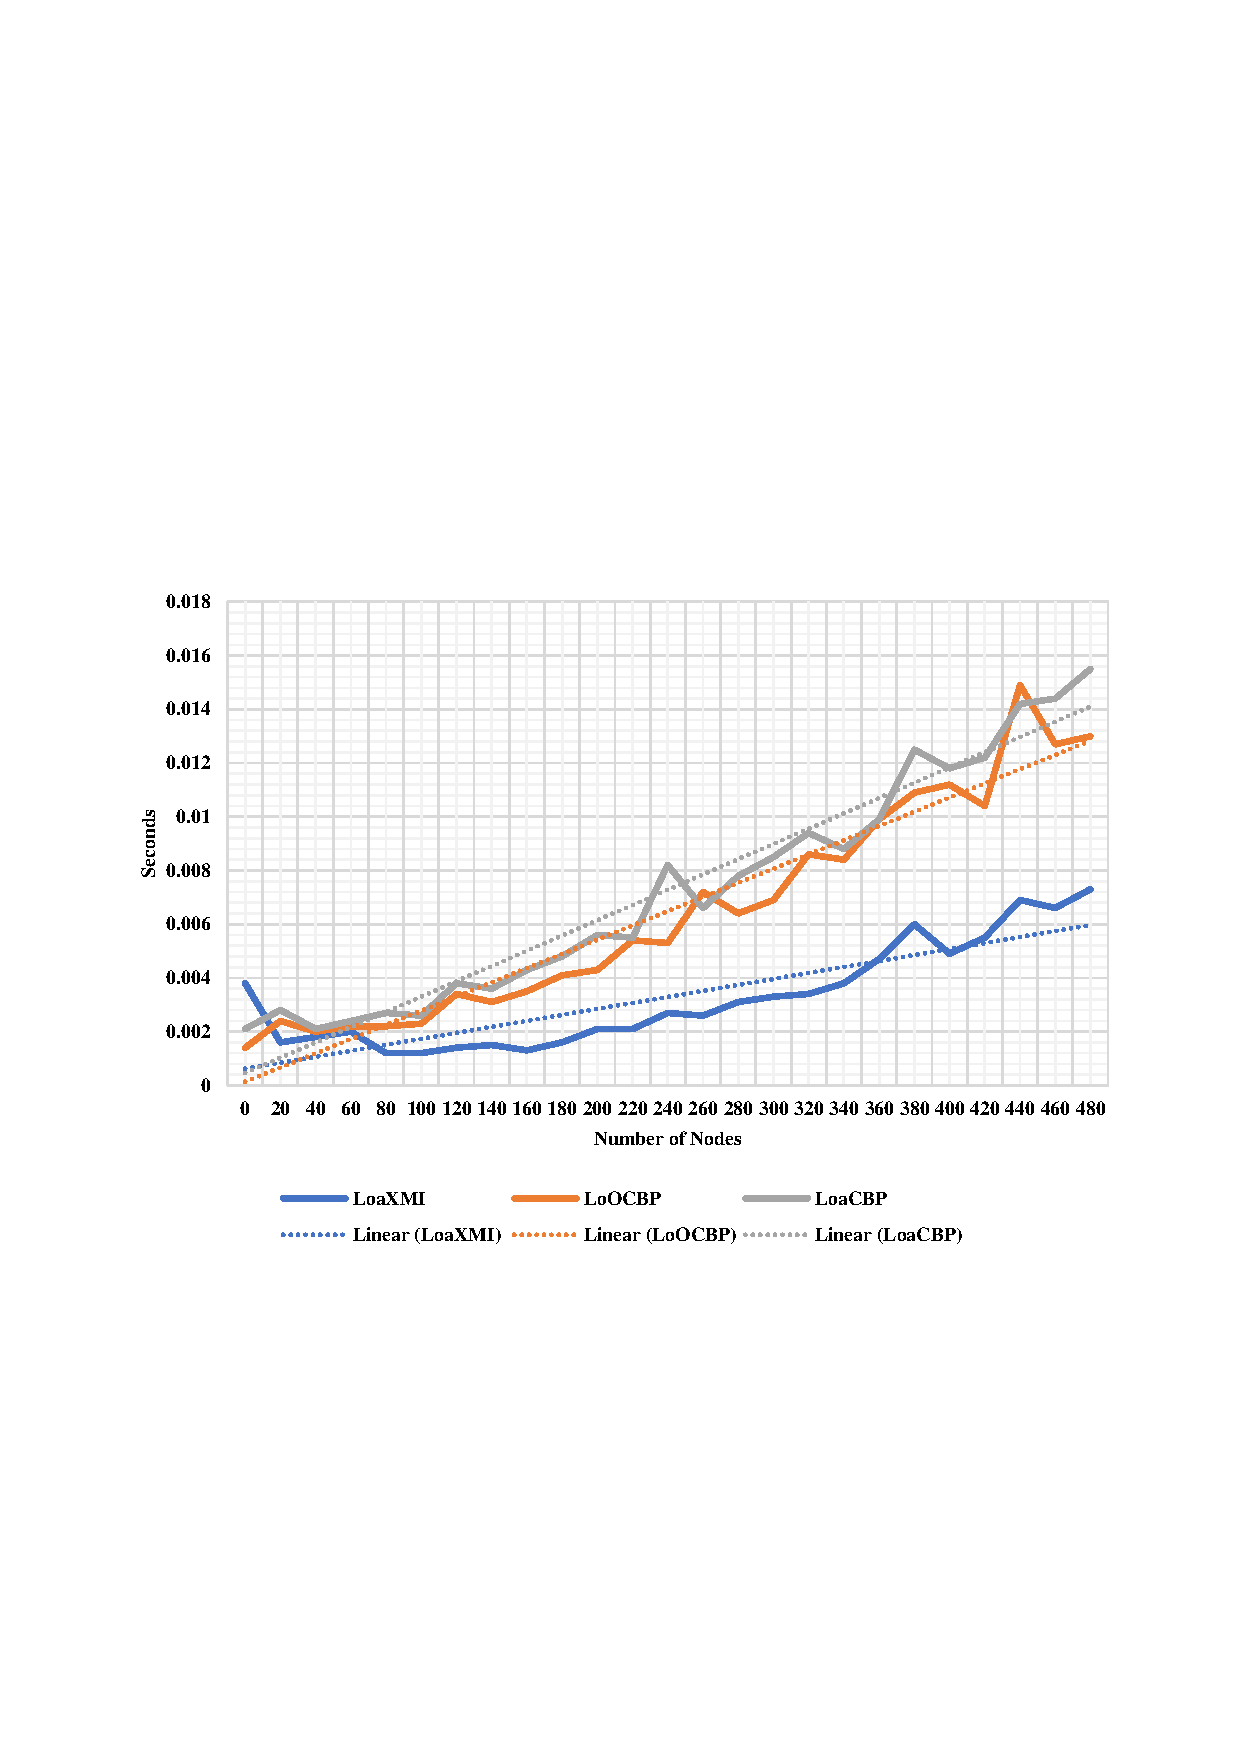
\includegraphics[width=\linewidth]{deep_tree}
\caption{Loading performance between loading XMI, optimised CBP, and CBP.}
\label{fig:deep_tree}
\end{figure}

\section{Related Work}

\section{Conclusions}


\cite{Lamport:LaTeX}.


\begin{acks}

\end{acks}
